
\section{Performance Evaluation, Results, Discussion}

\textit{owners: Evan: graphs, All: interpretation (2.75 pages)}
\begin{itemize}
  \item One graph showing benefits of various schemes for single-node scaling (cache, SIMD, etc.) [Fix the dataset -- $10^9$ nnzs?, Jatin will provide sample dataset]
  \item One scaling plot showing the following (Not sure if we have time to get scaling):
  \begin{itemize}
    \item Runtime for 4 CX phases
    \item Fix 1TB sized dataset
    \item Run on 960, 1920, 3840 cores on EC2  
  \end{itemize}

  \item One graph showing the following:
  \begin{itemize}
    \item EC2, Edison and Athena times
    \item 100GB and 1TB sized dataset
    \item stacked plot corresponding to all 4 phases
    \begin{figure} [h]
    \begin{centering}
    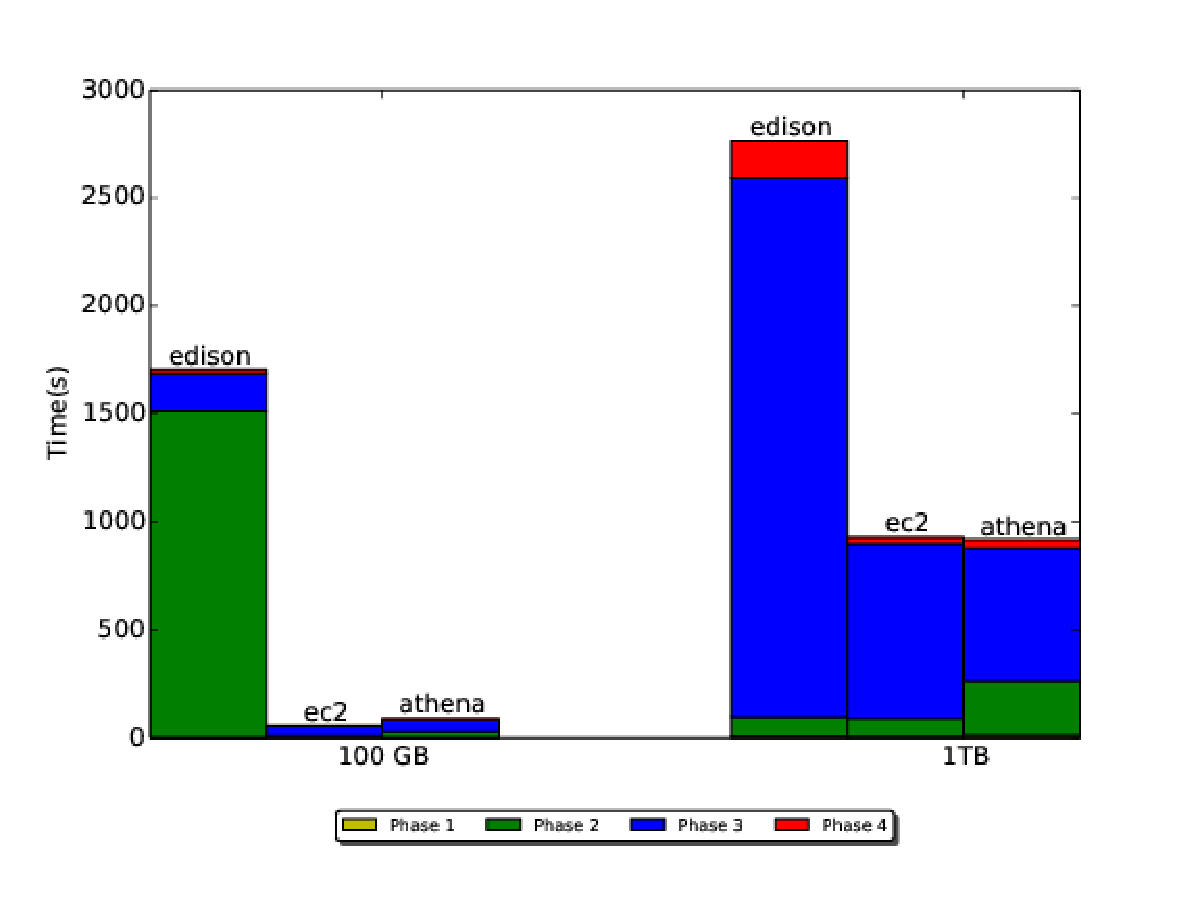
\includegraphics[scale=0.4]{images/CX_Size_Scaling}
    \end{centering}
    \caption{ Run times for the various stages of computation for CX for two different dataset sizes for the three platforms using rank 32 and default partitioning for the given platform} 
    \end{figure}
   
  \end{itemize}
 \item Comparison of CX, PCA, RPCA quantitatively (Alex will work on this)? 
  \begin{itemize}
    \item (for 100GB sized dataset on EC2)
    \item runtime vs. accuracy?
    \item show distinction b/w cx, pca
    \item alex will take ownership
  \end{itemize}

 \item Science plot for PCA, CX (Jiyan and Oliver will produce this)
\end{itemize}
